% !TeX root = ./report.tex

\documentclass{IEEEtran}
\usepackage{bm}
\usepackage{amsmath}
\usepackage{amssymb}
\usepackage{booktabs}
\usepackage{algorithm}
\usepackage{algorithmicx}
\usepackage{algpseudocode}
\usepackage{footnote}
\usepackage{stfloats}
\usepackage{graphicx}
\usepackage{url}
\DeclareMathOperator*{\argmax}{arg\,max}
\DeclareMathOperator*{\argmin}{arg\,min}
\makesavenoteenv{figure}
\title{Title}
\author{
    Fan~JIN
    \thanks{Fan~JIN 2015011506  \texttt{jinf15@mails.tsinghua.edu.cn}}
}

\begin{document}
\maketitle
\begin{abstract}
    Abstract
\end{abstract}
\begin{IEEEkeywords}
    Keywords 1, Keywords 2,
\end{IEEEkeywords}

\section{Question 1: Function Optimization}
{
    \subsection{Target function: Eggholder}
    {
        As intelligent optimization algorithms have emerged as a new paradigm of function optimization, 
        many test functions have been proposed to serve as benchmarks \cite{wiki:Test_functions_for_optimization}.
        In this report, the Eggholder function is chosen to test two intelligent optimization algorithms:
        the simulated annealing (SA) and the differential evolution (DE).

        The Eggholder function is defined as
        \[
            \begin{split}
            f(x,y) &= \\
            &- (y+47) \sin{\sqrt{\left| \frac{x}{2}+(y+47) \right|}} \\
            &- x \sin{\sqrt{\left| x-(y+47) \right|}},
            \end{split}
        \]
        where $-512 < x,y < 512$.
        Its global minimum is known as $f(512, 404.2319) = -959.6407$. (Figure \ref{fig:eggholder})

        \begin{figure}[!htbp]
            \centering
            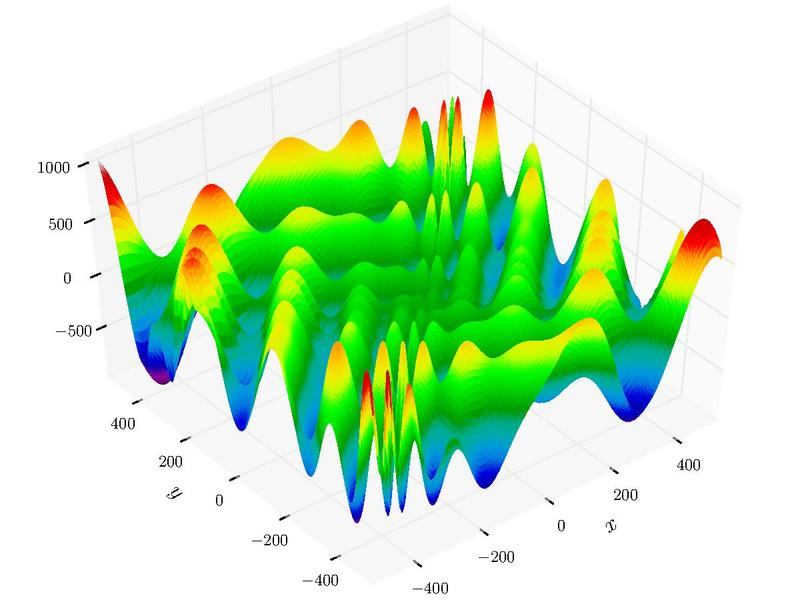
\includegraphics[width=0.45\textwidth]{figures/eggholder.png}
            \caption{Eggholder function \cite{wiki:Test_functions_for_optimization}}
            \label{fig:eggholder}
        \end{figure}

        Eggholder function is challenging bacause 
        i) it has boundary constraints on both $x$ and $y$, and 
        ii) the global minimum is at the boundary of $x=512$, and 
        iii) there are dozens of local minimums throughout the space.
        
    }

    \subsection{Implementation of SA and DE}
    {
        \begin{figure}[!htbp]
            \centering
            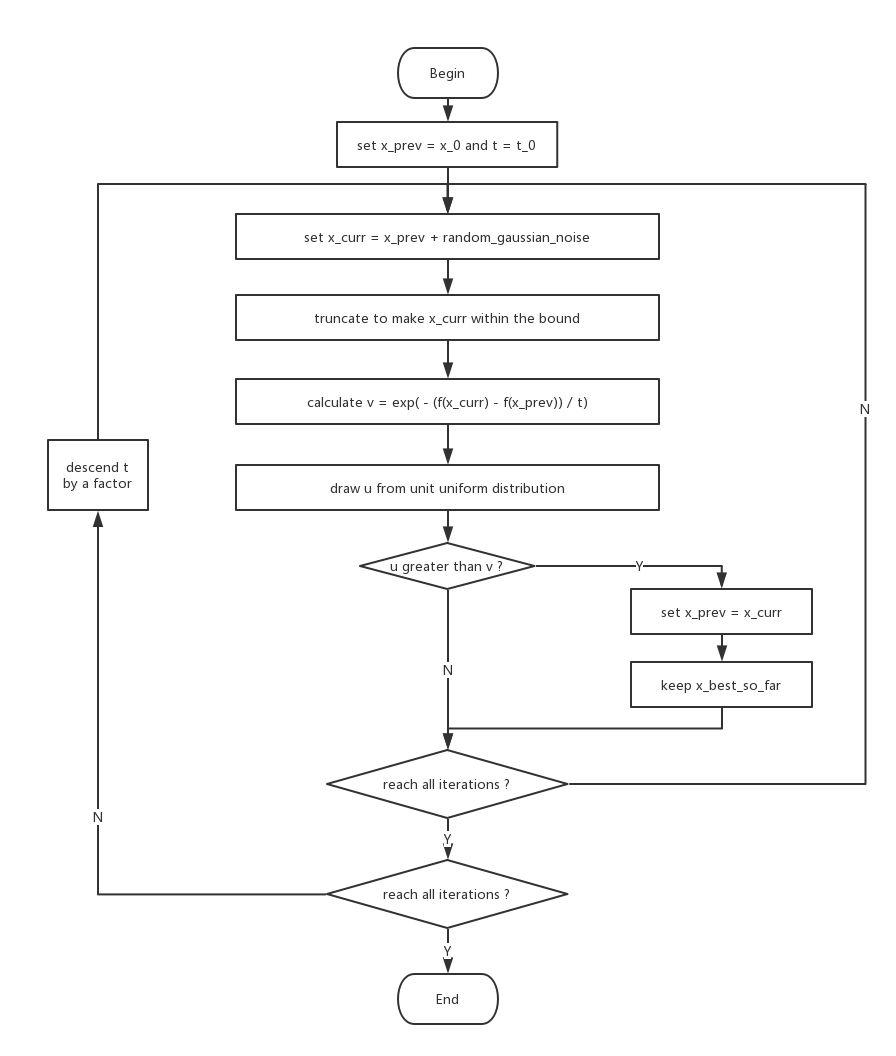
\includegraphics[width=0.45\textwidth]{figures/SA_algorithm.png}
            \caption{Flow chart of simulated annealing (SA)}
            \label{fig:SA}
        \end{figure}

        \begin{figure}[!htbp]
            \centering
            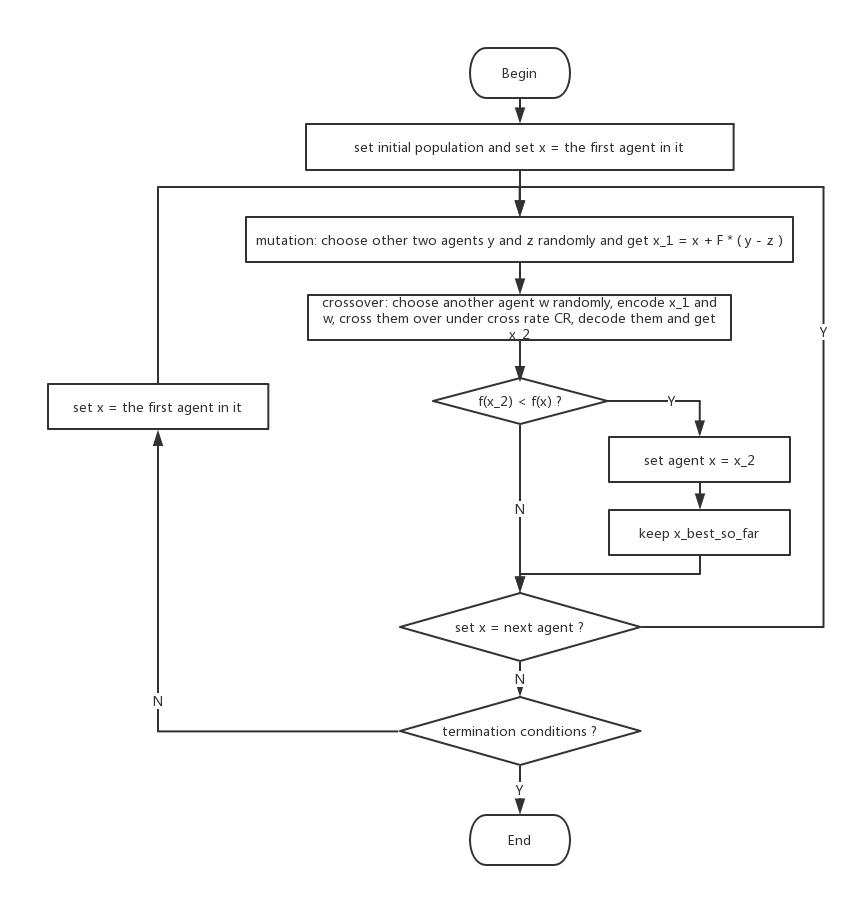
\includegraphics[width=0.45\textwidth]{figures/DE_algorithm.png}
            \caption{Flow chart of differential evolution (DE)}
            \label{fig:DE}
        \end{figure}

        To make full use of vectorized operations in MATLAB, we use ``arrayfun'' function to evaluate the target function in batches. 
        The ``encode'' and ``decode'' functions are also written using vectorized operations to gain more performance. 
        (Figure \ref{fig:SA} and \ref{fig:DE})
    }

    \subsection{Experiments}
    {
        \subsubsection{The trivial sphere function}
        {
            The sphere function is quite trivial. 
            Defined as
            $$f(x, y) = x^2 + y^2,$$
            it is convex and has no local minimums but a global minimum.

            We tested our SA and DE implementations on sphere function. 
            The result shows that the algorithms we implemented give the global minimum with convergence as expected. 
            (Figure \ref{fig:sphere_SA} and \ref{fig:sphere_DE})

            \begin{figure}[!htbp]
                \centering
                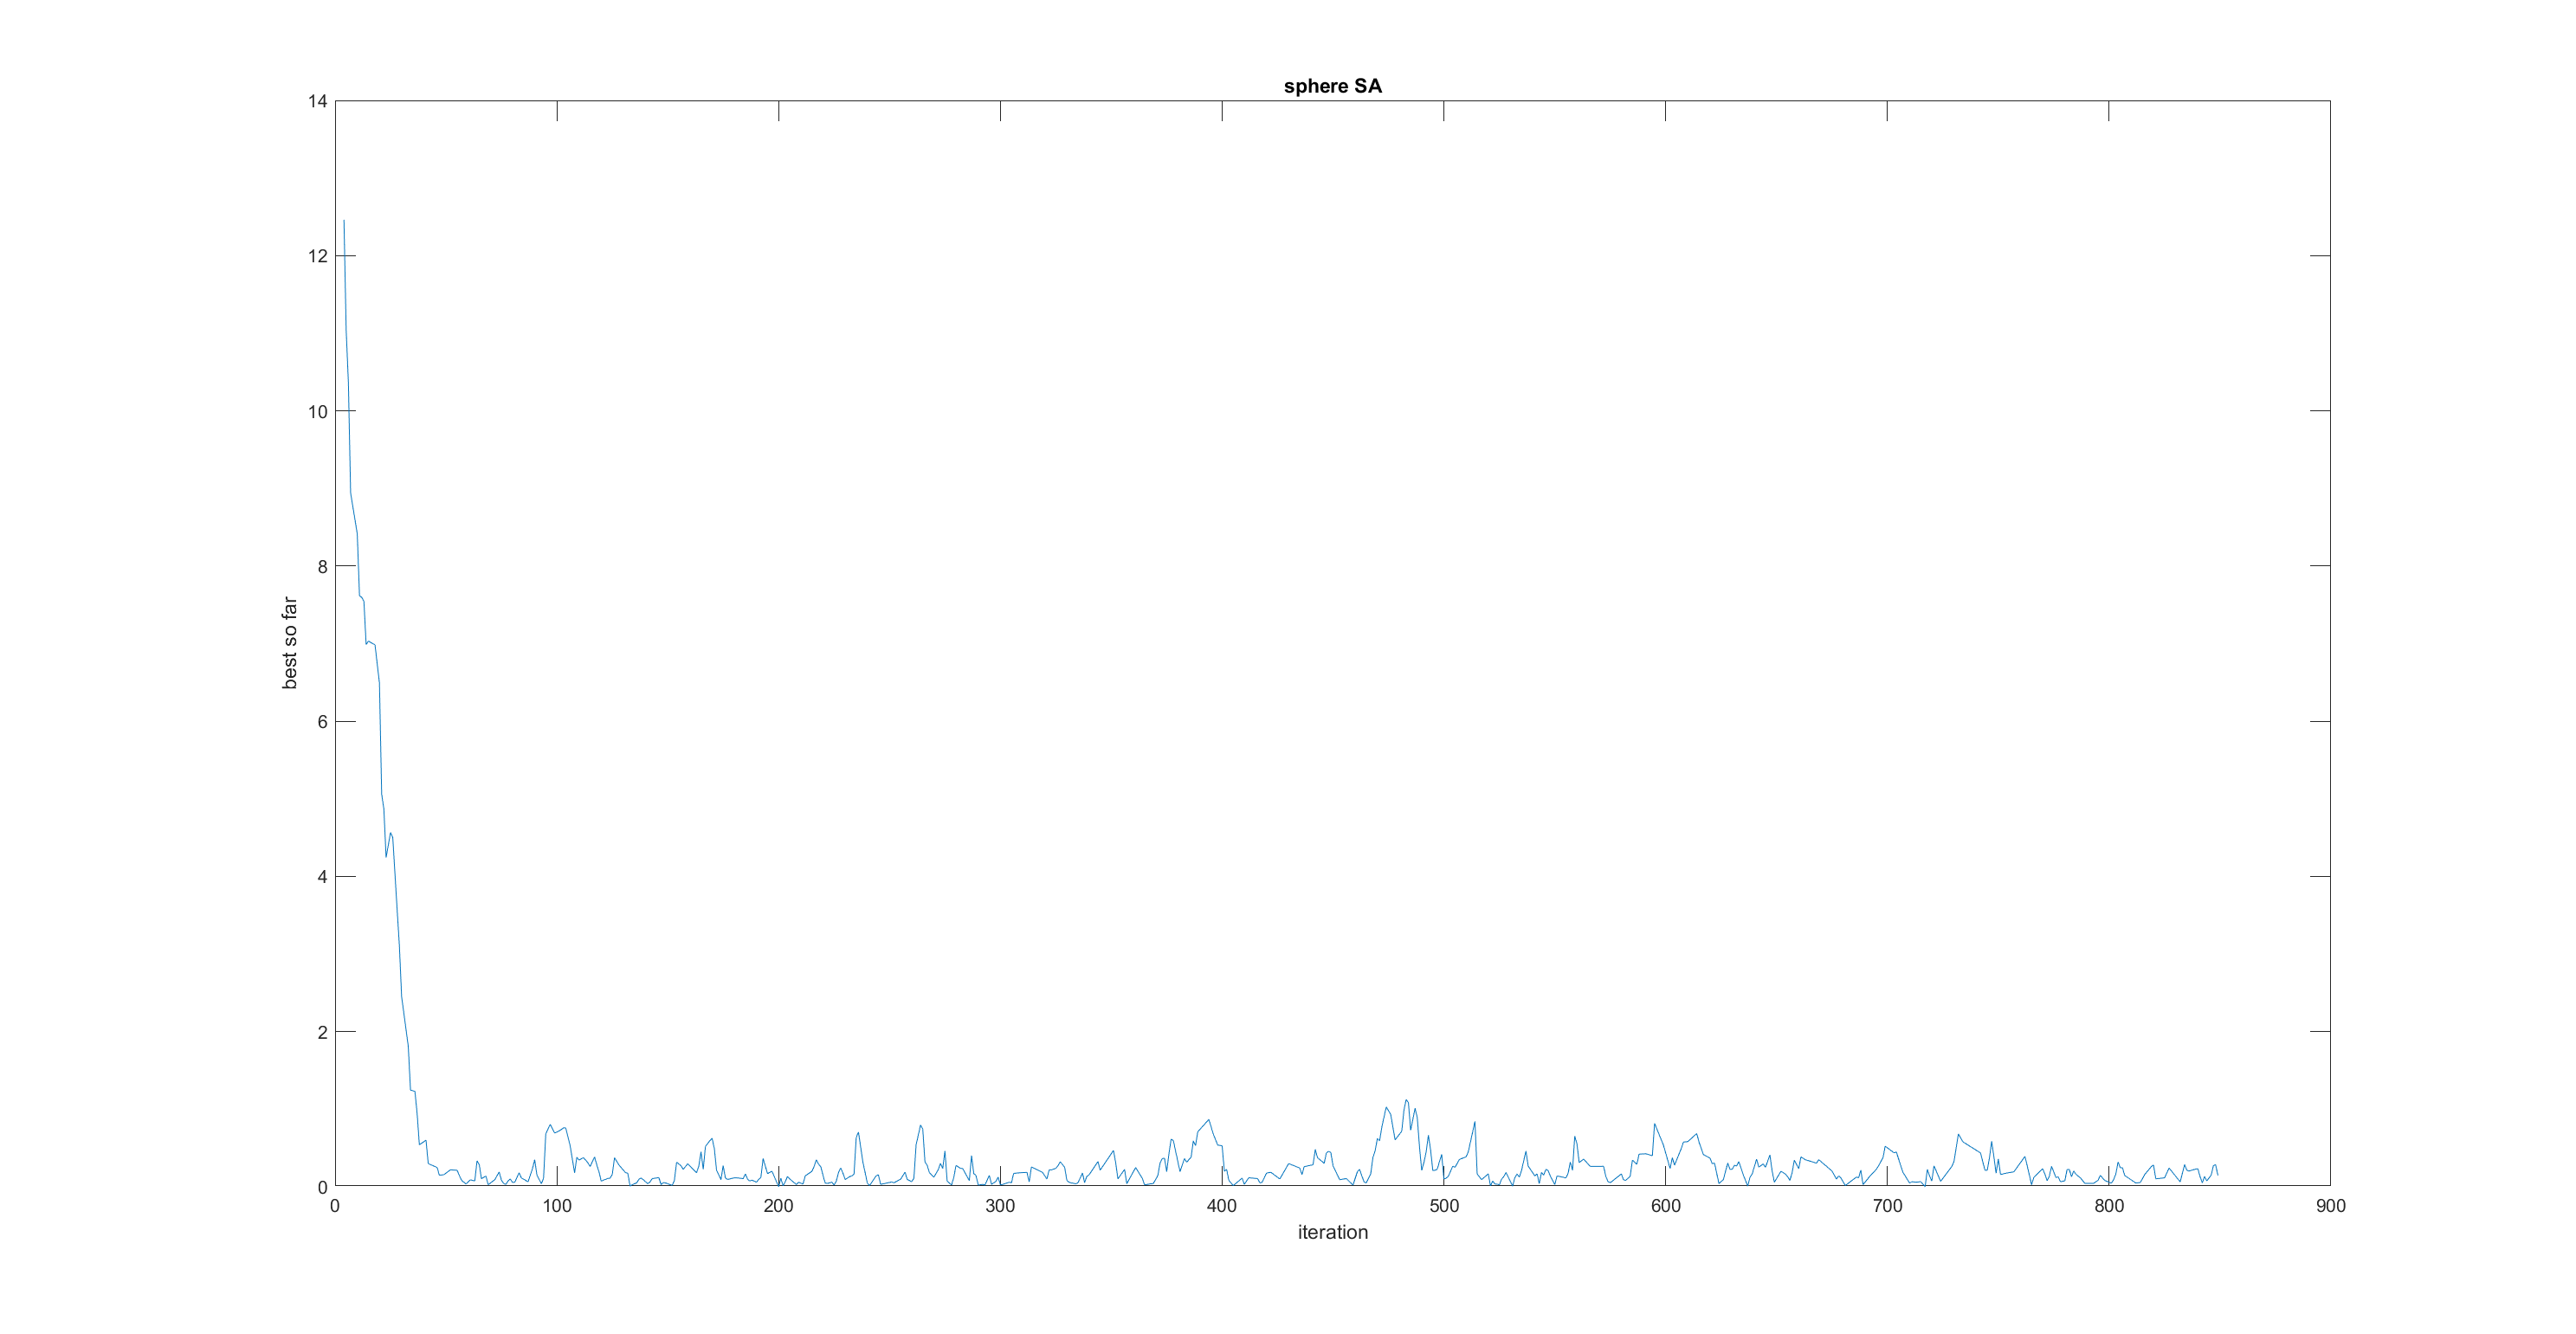
\includegraphics[width=0.45\textwidth]{Q1/figures/sphere_SA.png}
                \caption{Performance of SA on the sphere function}
                \label{fig:sphere_SA}
            \end{figure}

            \begin{figure}[!htbp]
                \centering
                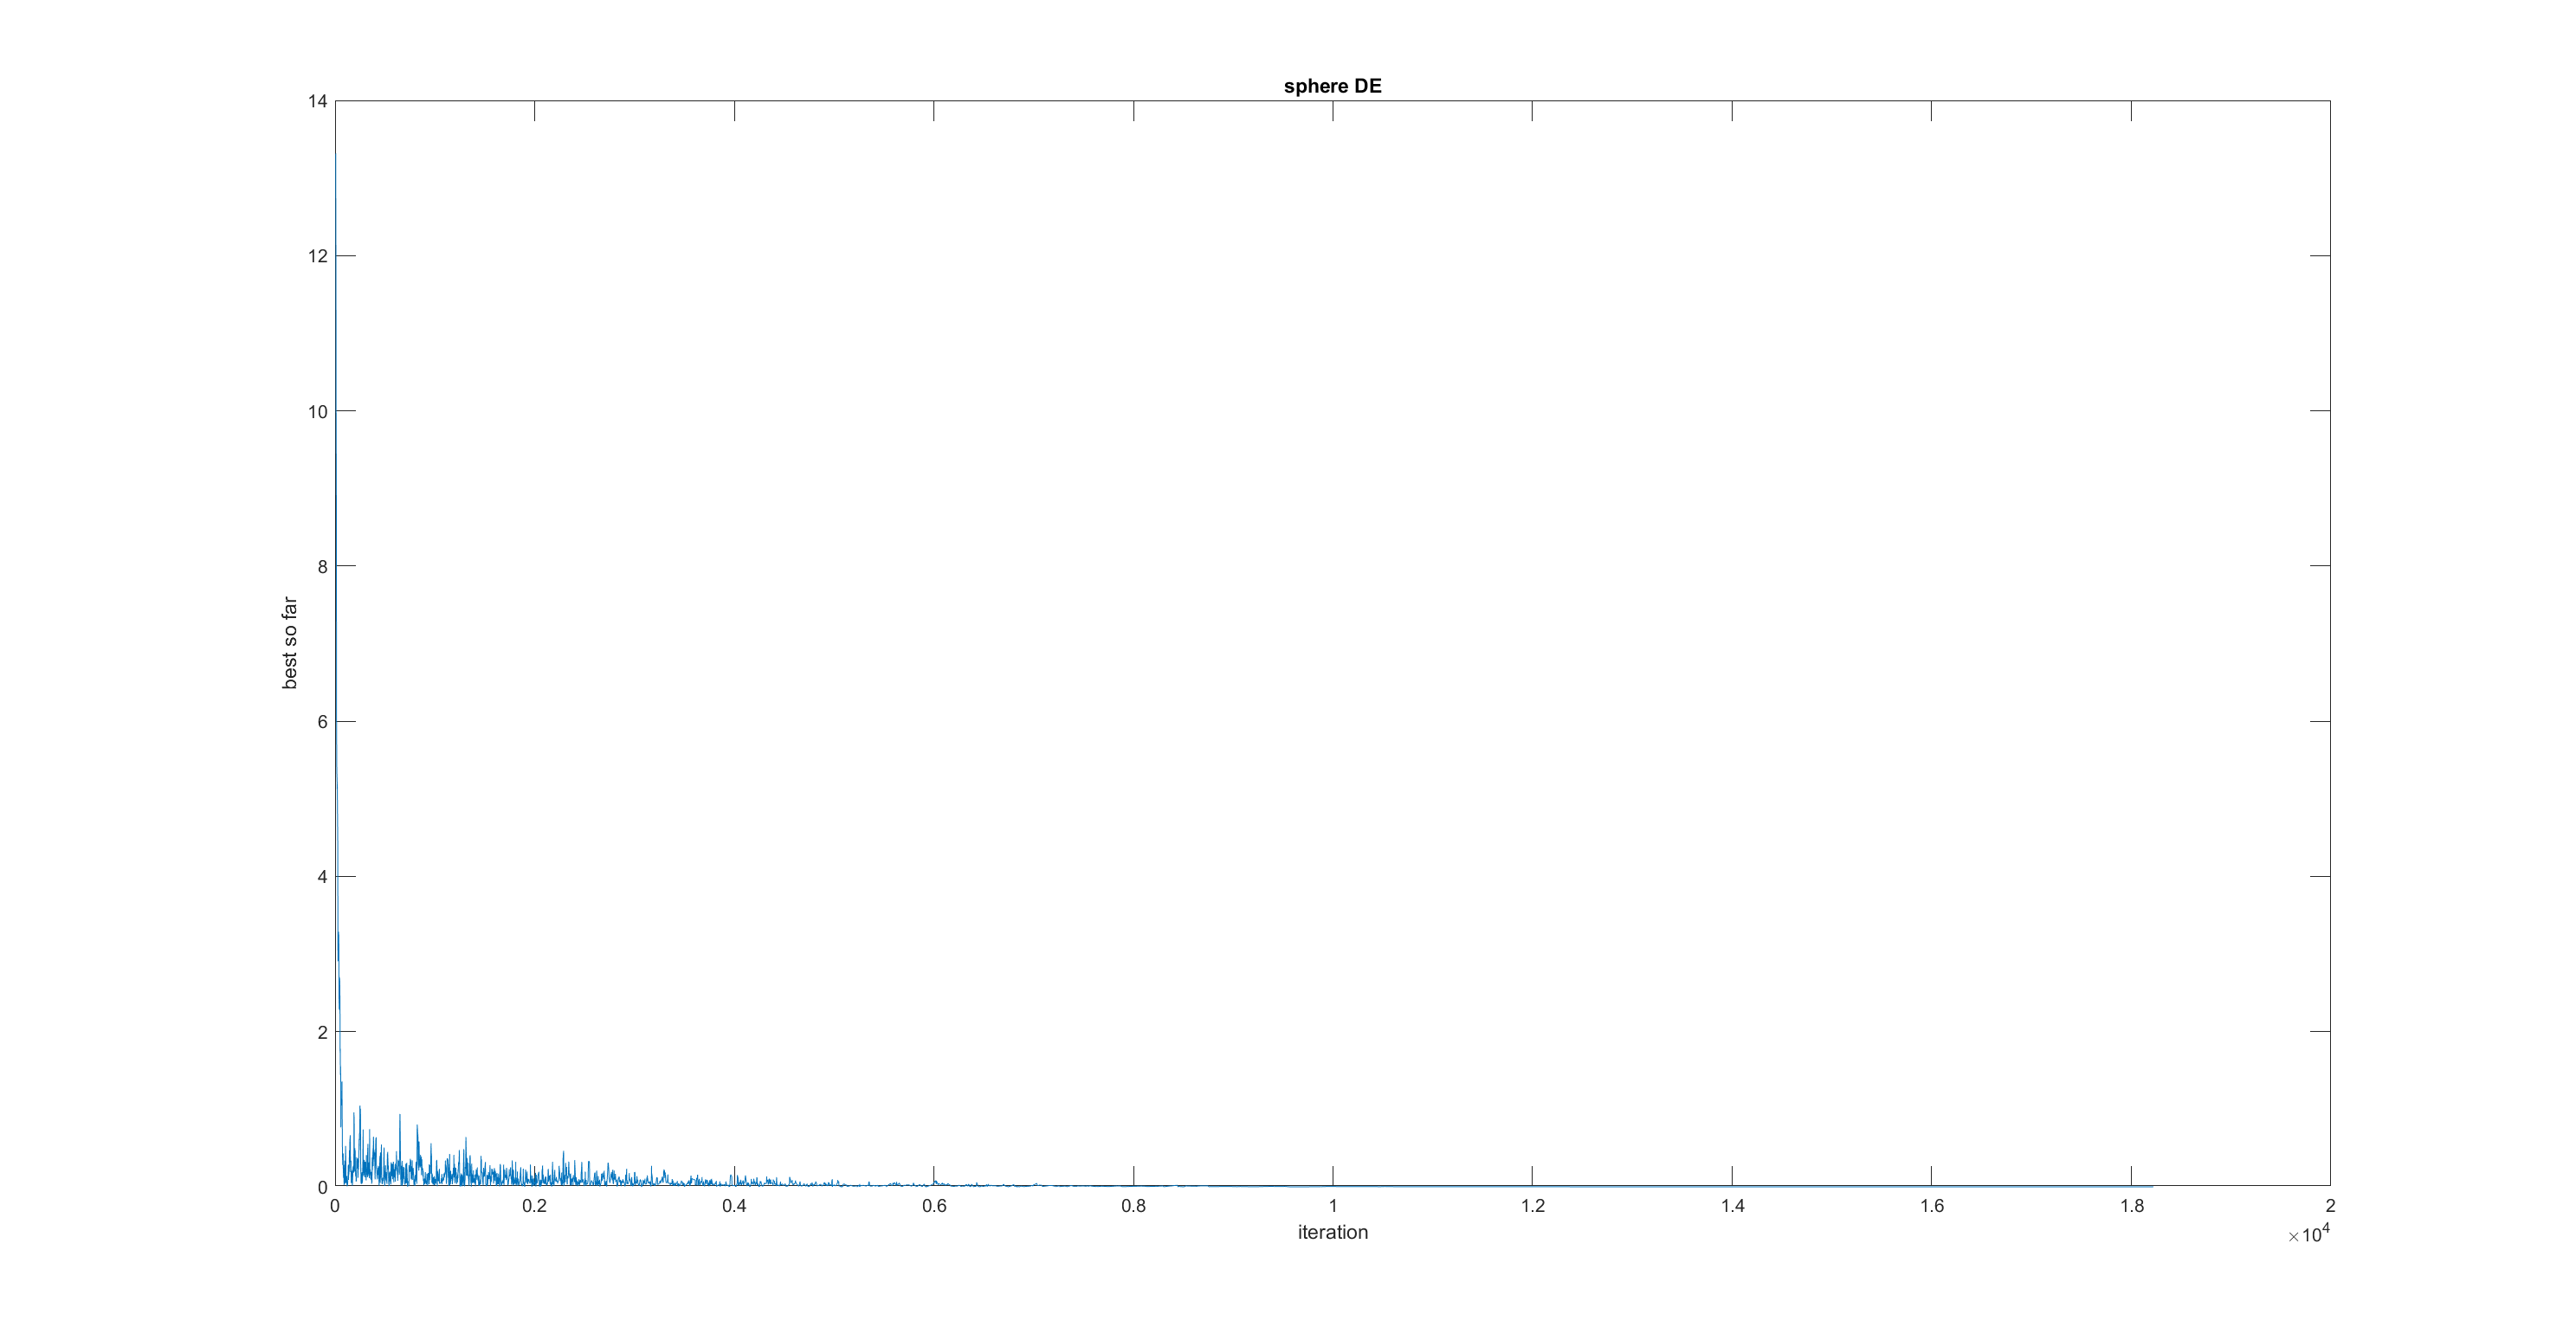
\includegraphics[width=0.45\textwidth]{Q1/figures/sphere_DE.png}
                \caption{Performance of DE on the sphere function}
                \label{fig:sphere_DE}
            \end{figure}
        }

        \subsubsection{The eggholder function}
        {
            Repeated for 20 times, the performance (best value searched and time cost) of each algorithm is recorded. 
            (Table \ref{tab:performance_Q1} and \ref{tab:timecost_Q1})
            (Figure \ref{fig:eggholder_SA} and \ref{fig:eggholder_DE})

            \begin{table}[!hbp]
                \centering
                \begin{tabular}{|c|c|c|c|}
                    \hline
                    Alg. & best so far (min) & b.s.f. (mean) & b.s.f. (max) \\
                    \hline
                    SA &  -959.6406 &  -872.9803 &  -555.5534 \\
                    \hline
                    DE &  -959.6407 &  -959.6404 &  -959.6386 \\
                    \hline
                \end{tabular}
                \caption{Performance after 20th repitition}
                \label{tab:performance_Q1}
            \end{table}

            \begin{table}[!hbp]
                \centering
                \begin{tabular}{|c|c|c|c|}
                    \hline
                    Alg. & time cost in sec (min) & t.c. (mean) & t.c. (max) \\
                    \hline
                    SA &  0 &  0.0055 &  0.0469 \\
                    \hline
                    DE &  5.2656 &  6.6070 &  8.9688 \\
                    \hline
                \end{tabular}
                \caption{Time cost after 20th repitition}
                \label{tab:timecost_Q1}
            \end{table}

            \begin{figure}[!htbp]
                \centering
                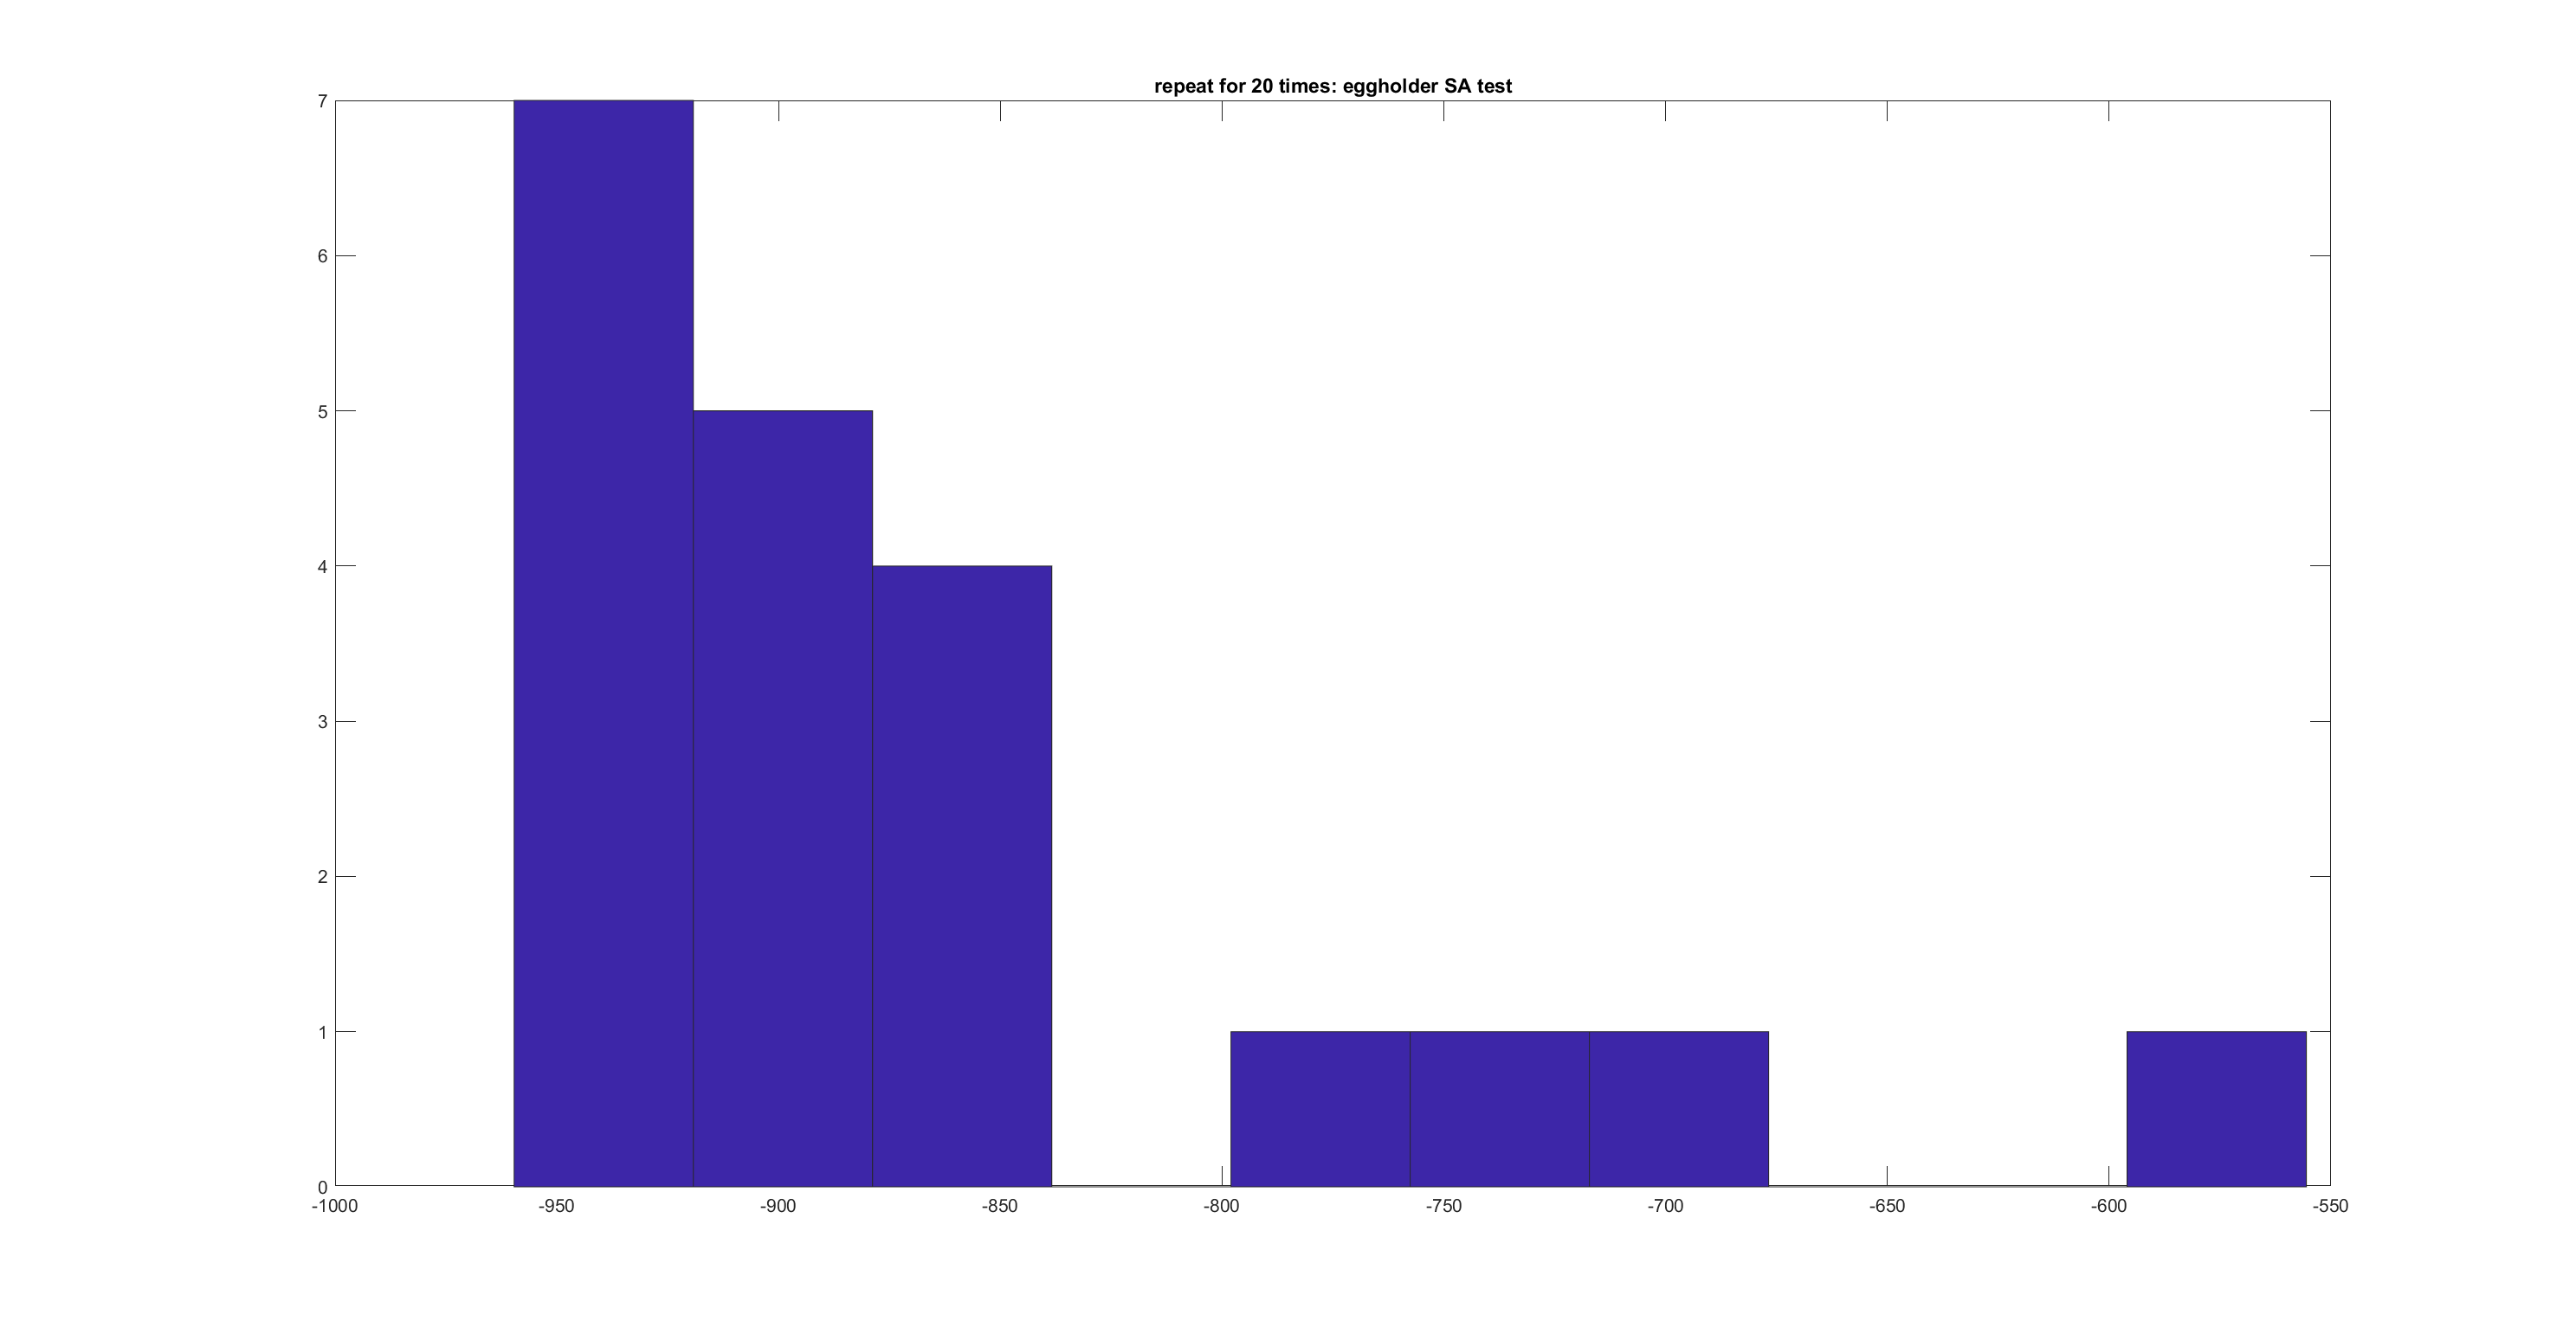
\includegraphics[width=0.45\textwidth]{Q1/figures/eggholder_SA_test.png}
                \caption{Performance of SA after 20th repitition}
                \label{fig:eggholder_SA}
            \end{figure}

            \begin{figure}[!htbp]
                \centering
                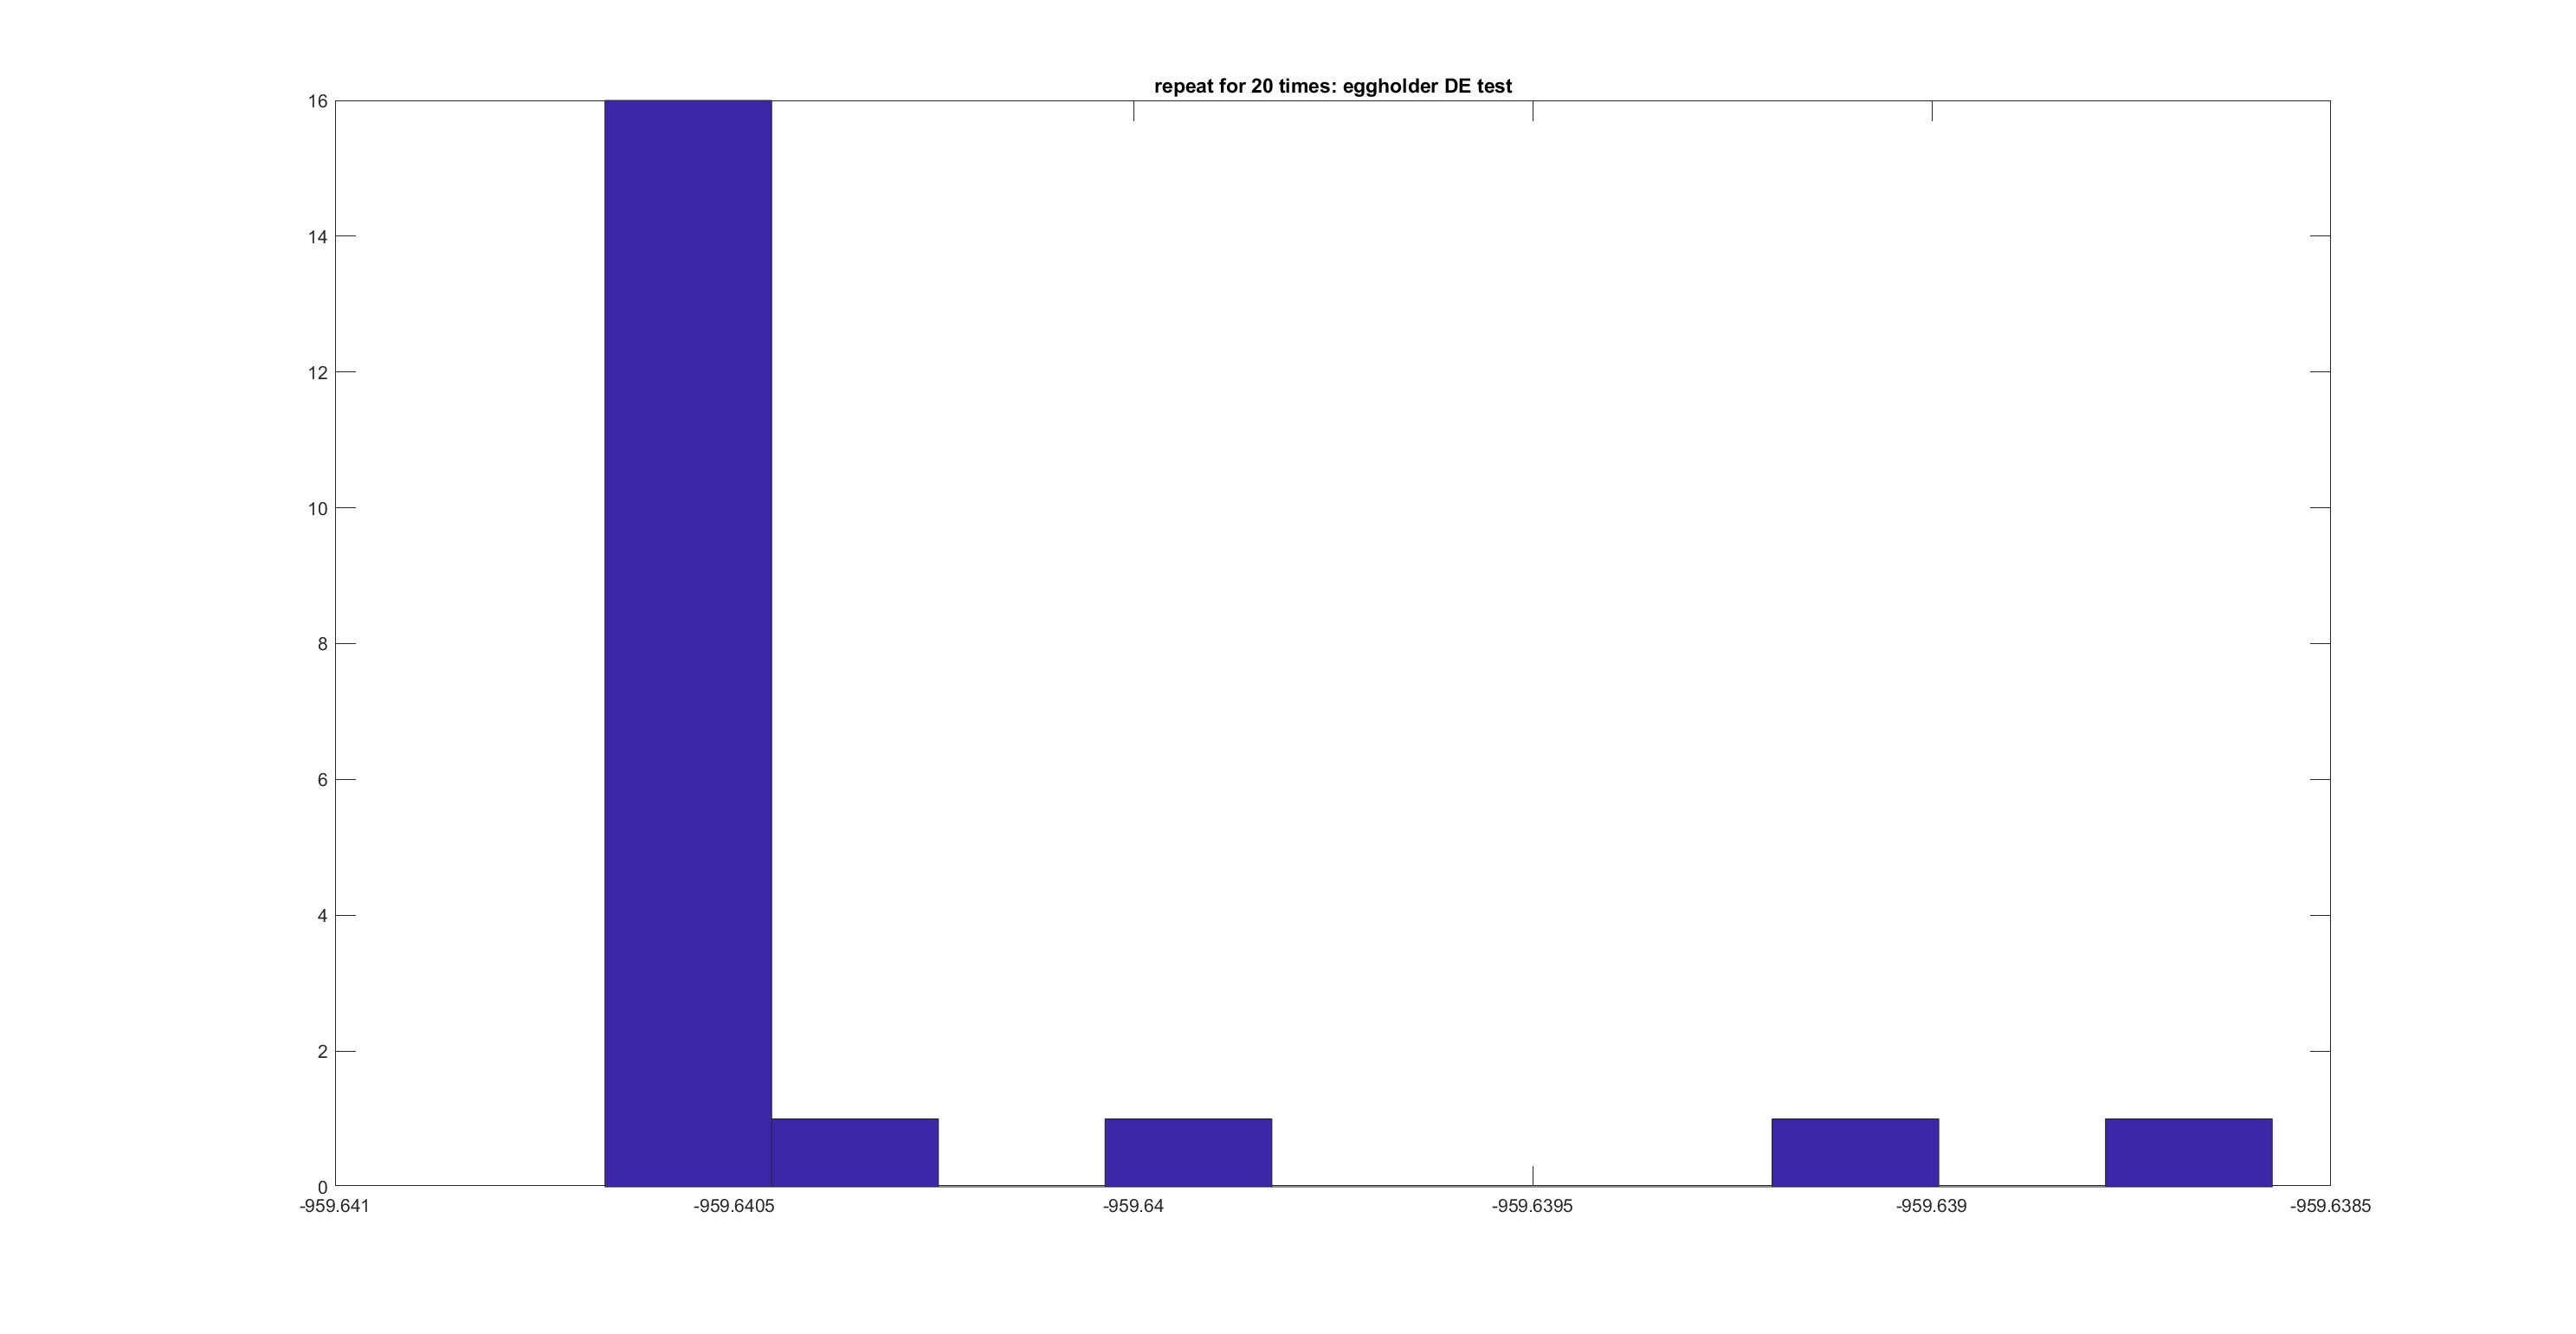
\includegraphics[width=0.45\textwidth]{Q1/figures/eggholder_DE_test.png}
                \caption{Performance of DE after 20th repitition}
                \label{fig:eggholder_DE}
            \end{figure}

            \begin{itemize}
                \item Performance: DE wins. DE always manages to find the global minimum at -959.64, while SA cannot. 
                Although SA did find the global minimum occasionally, the average performance is -872, which is still far from the best value.
                \item Time cost: SA wins. SA has little time cost, consuming 47 milliseconds in the worst case. 
                In contrast, it always takes seconds for DE to complete, because it is population-based rather than individual-based. 
                Obviously, the time cost of DE is proportional to the population size. 
                With a small population size, DE has a time cost affordable in certain circumstances.
            \end{itemize}
        }

        \subsubsection{Plots of best-so-fars}
        {
            \begin{figure}[!htbp]
                \centering
                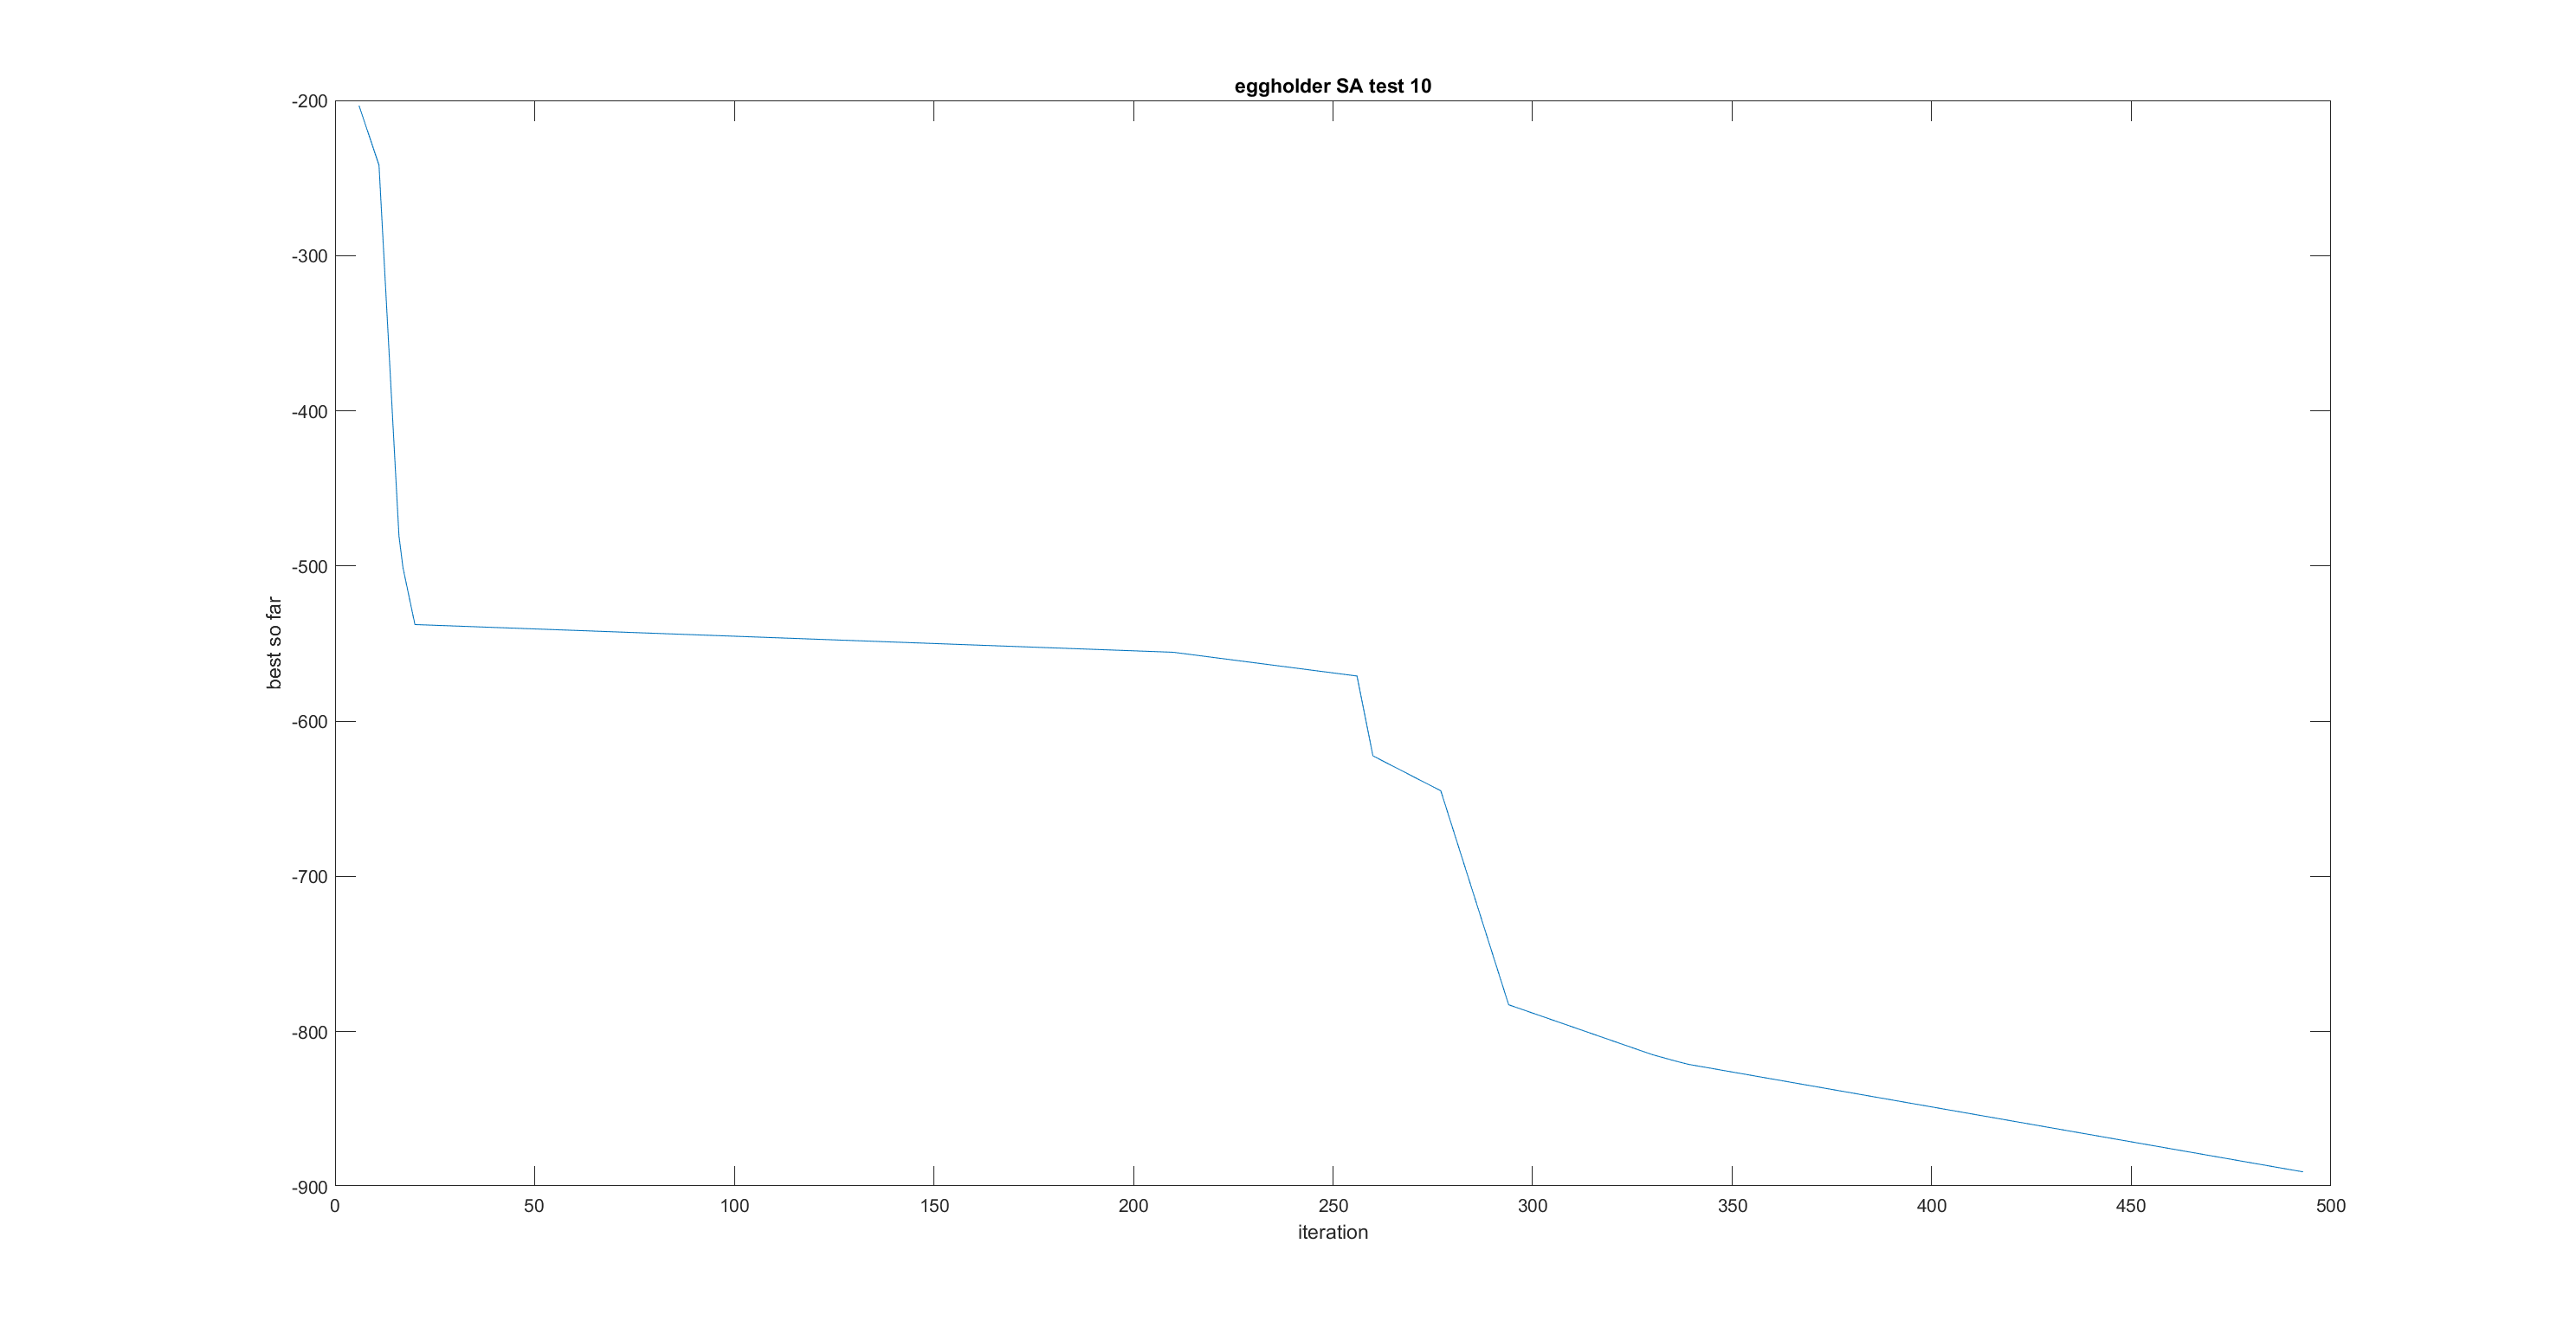
\includegraphics[width=0.45\textwidth]{Q1/figures/eggholder_SA_test_10.png}
                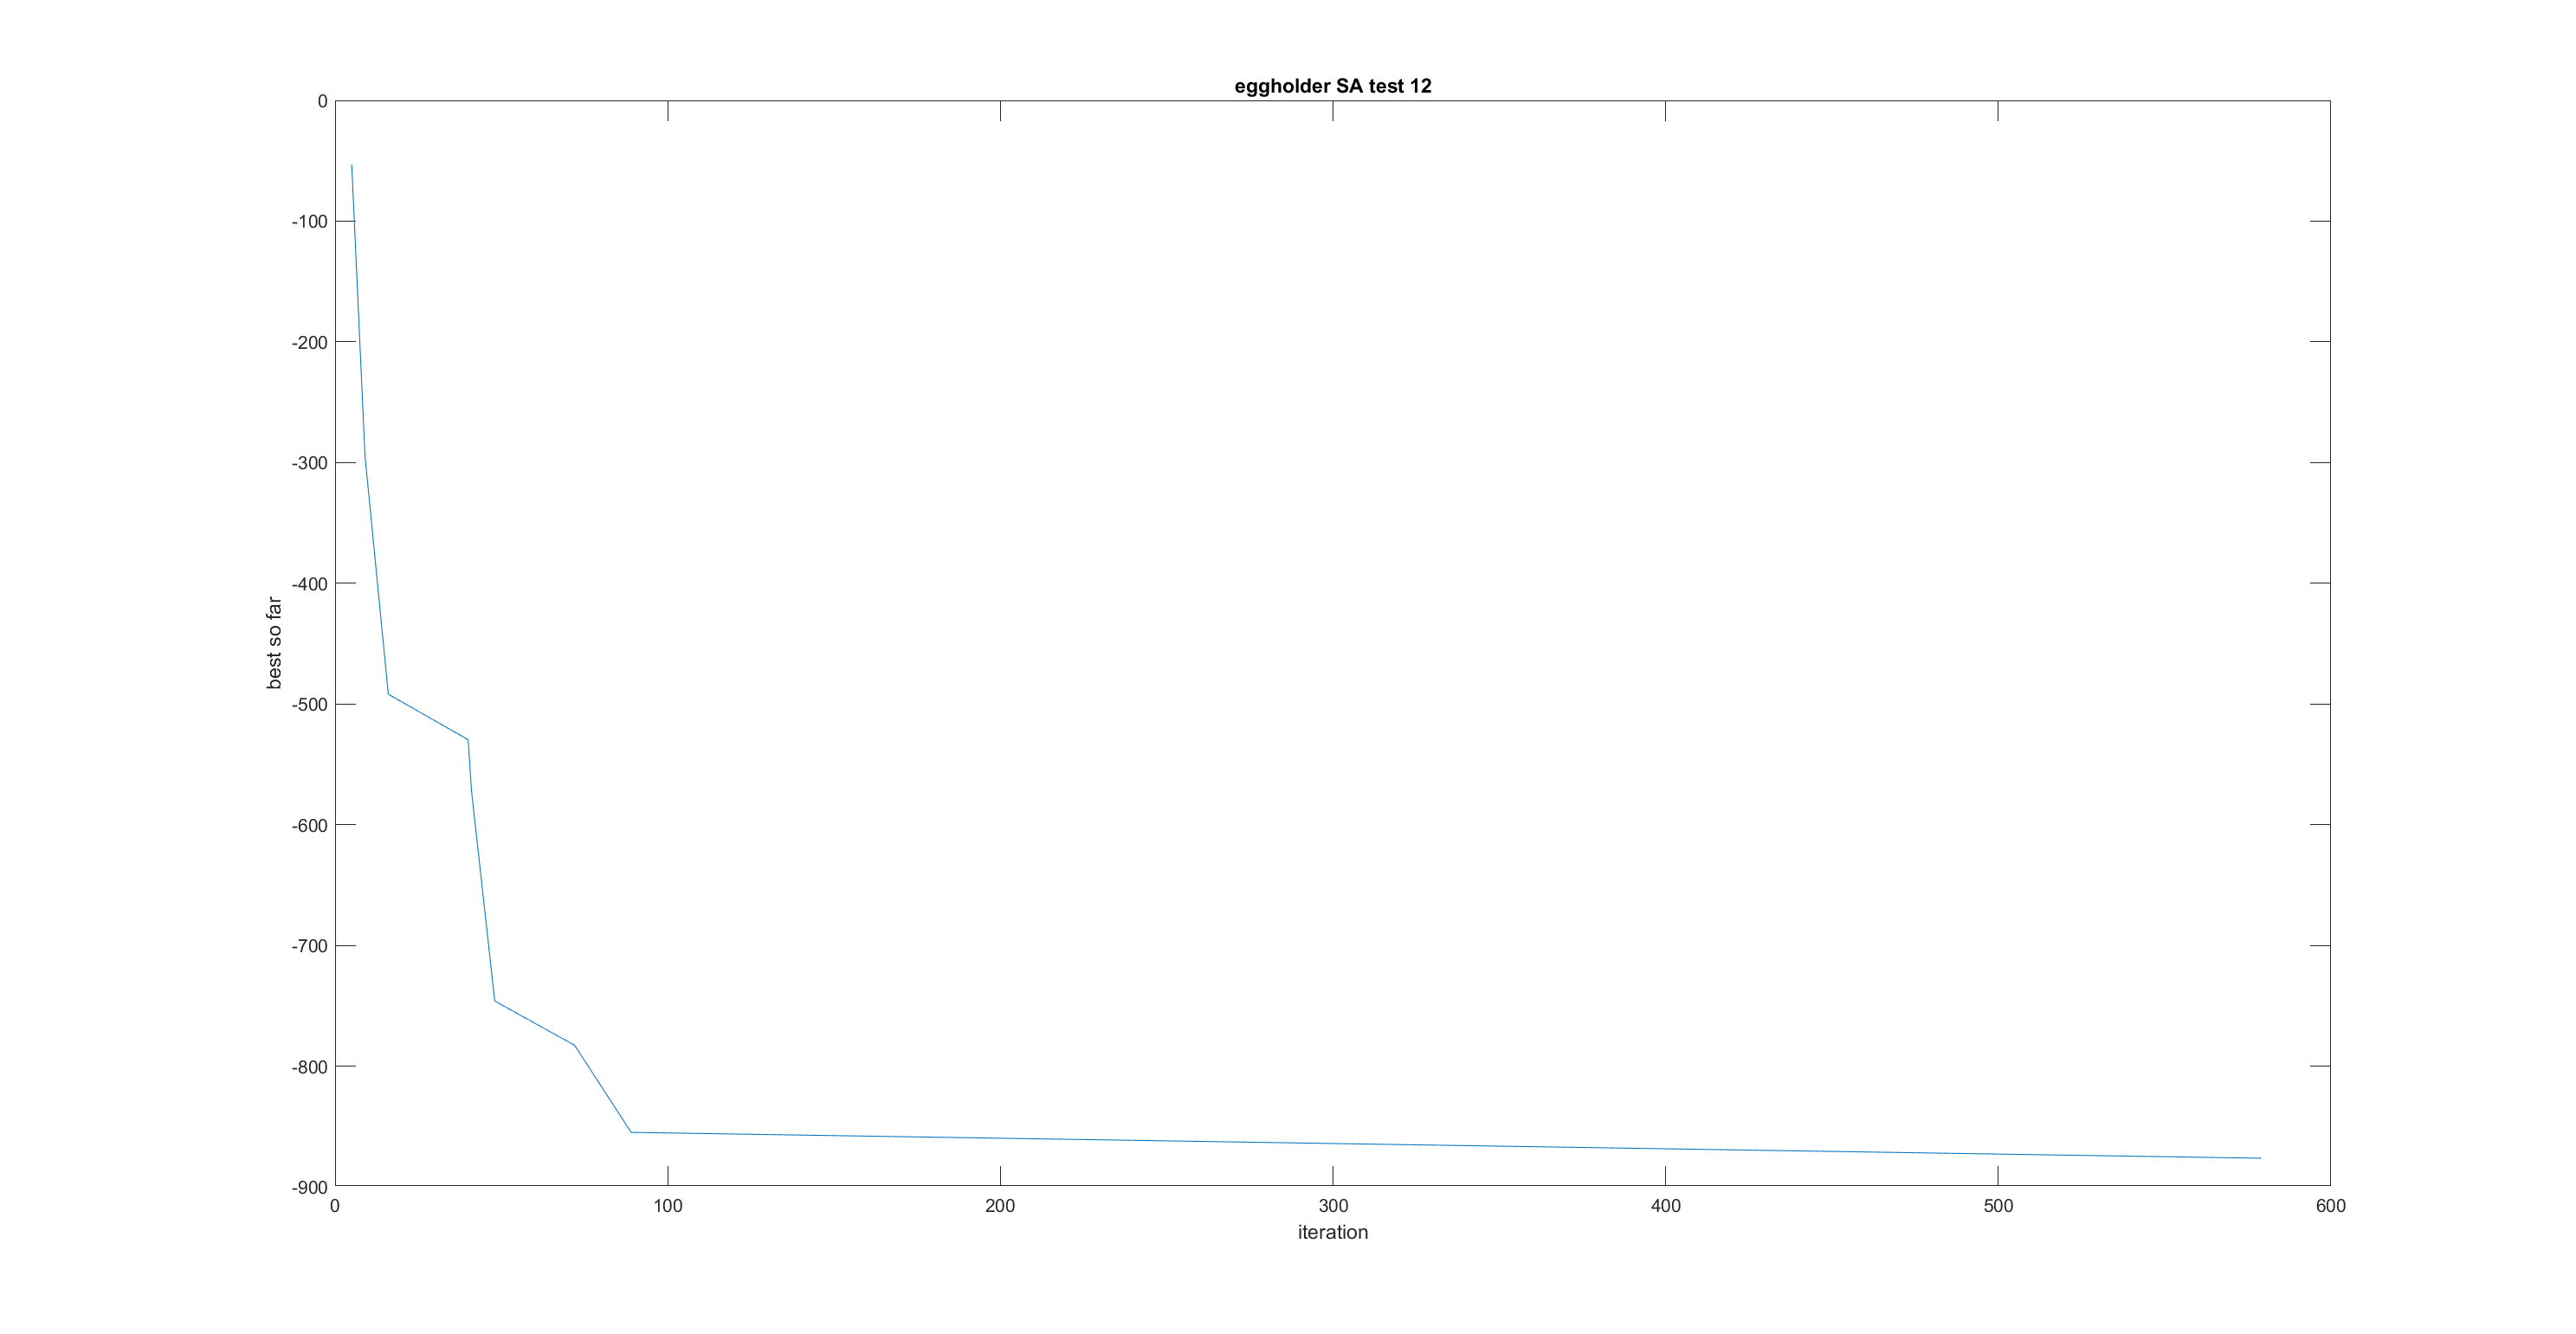
\includegraphics[width=0.45\textwidth]{Q1/figures/eggholder_SA_test_12.png}
                \caption{10th and 12th test of SA}
                \label{fig:plots_SA}
            \end{figure}

            \begin{figure}[!htbp]
                \centering
                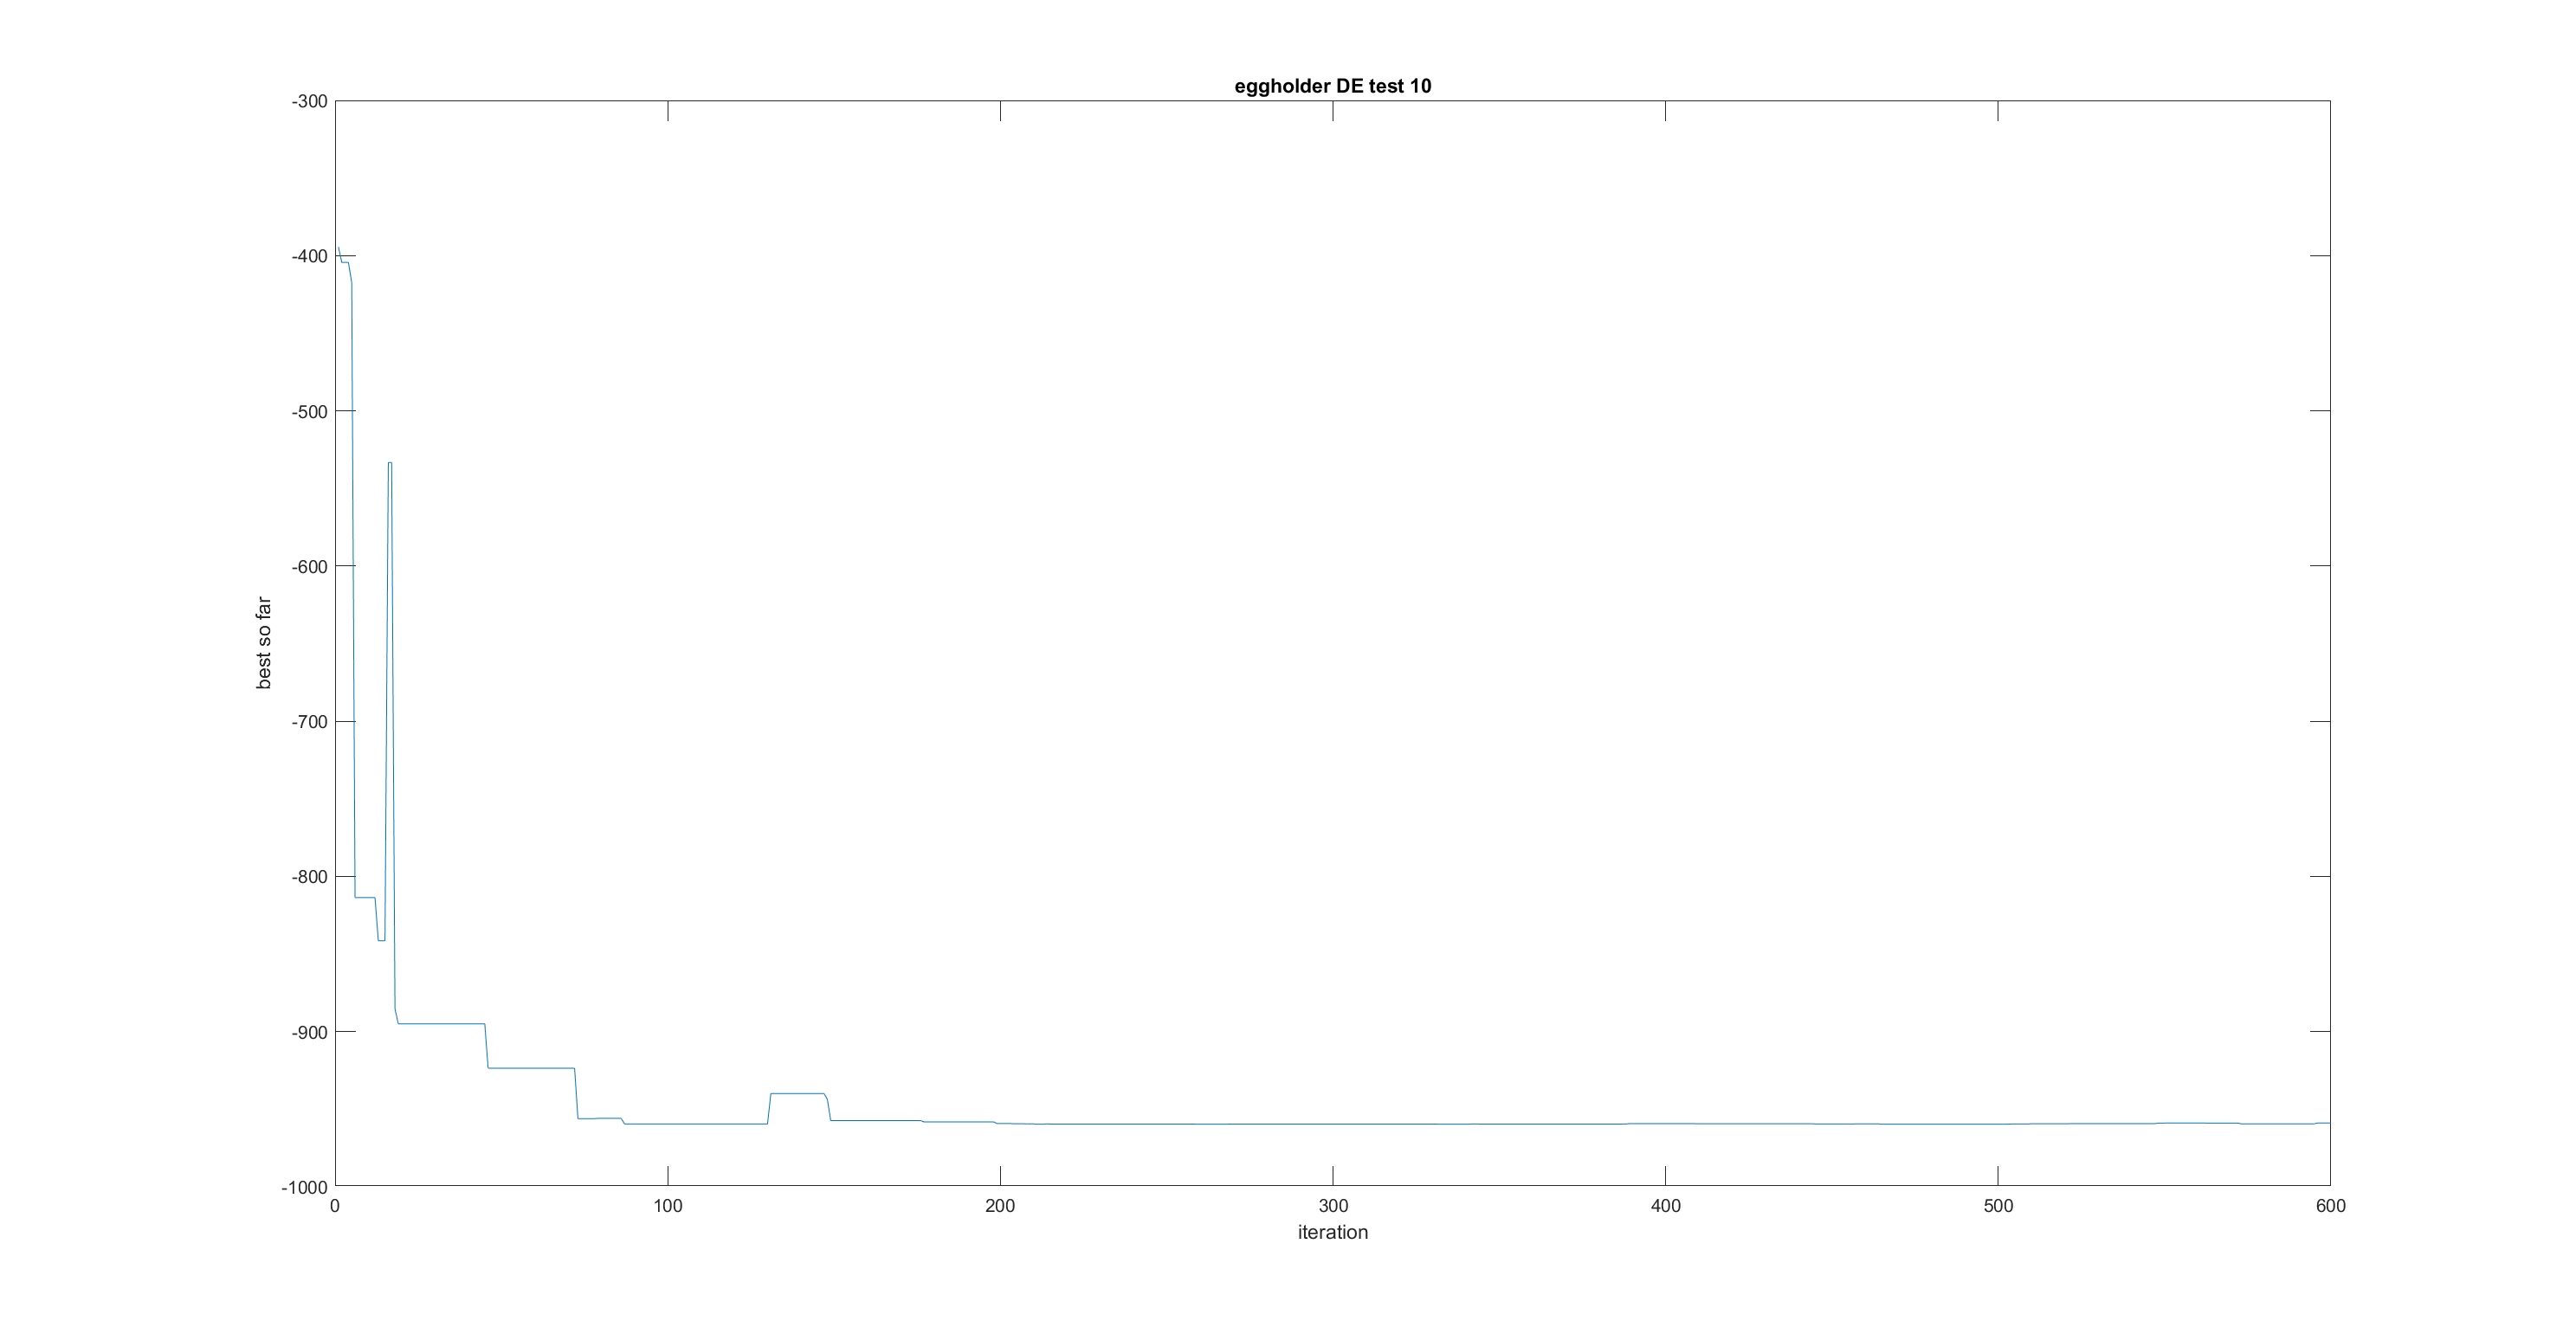
\includegraphics[width=0.45\textwidth]{Q1/figures/eggholder_DE_test_10.png}
                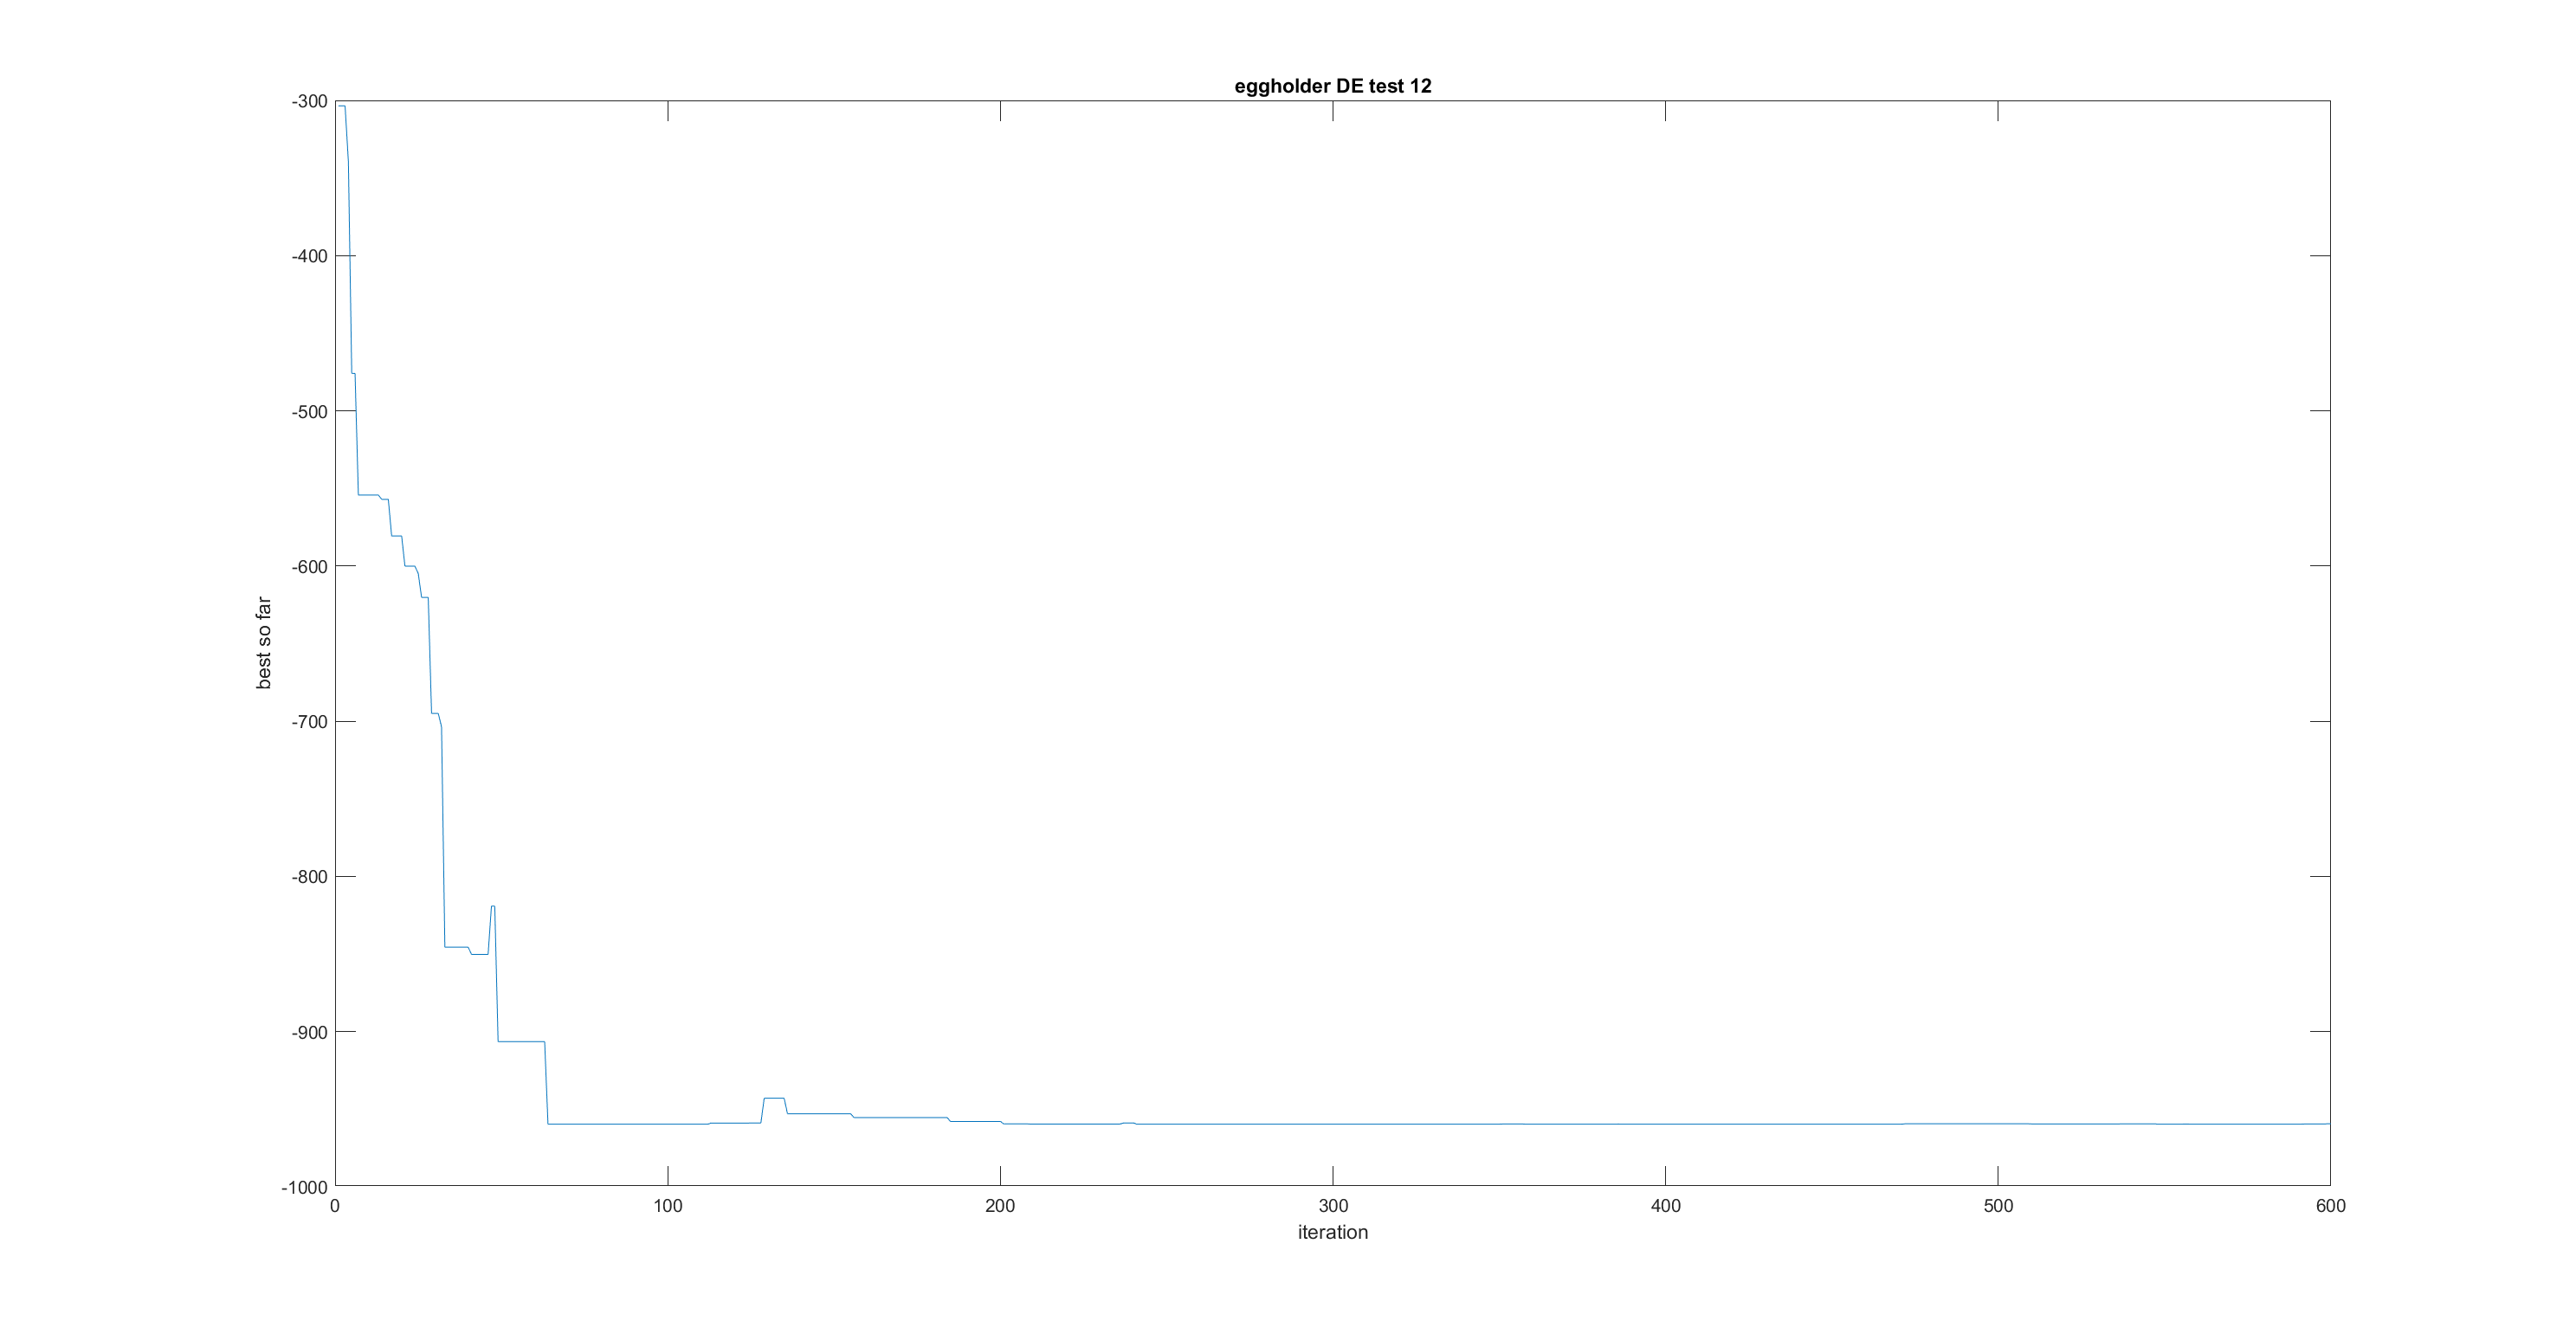
\includegraphics[width=0.45\textwidth]{Q1/figures/eggholder_DE_test_12.png}
                \caption{10th and 12th test of DE}
                \label{fig:plots_DE}
            \end{figure}

            From Figure \ref{fig:plots_SA} and \ref{fig:plots_DE}, we see that
            \begin{itemize}
                \item The number of iterations needed for SA varies a lot. For test 10, it took 400 epochs. For test 12, only 200 is enough.
                \item DE is much more stationary. Although it is not a monotonic descent, it converges very quickly.
            \end{itemize}
        }
    }

    \subsection{Sensitivity Analysis}
    {

    }
}

\bibliographystyle{ieeetran}
\bibliography{reference}
\end{document}